\chapter{Microarrays}
\label{c:microarrays}

\section{The dataset} \label{chapter_dataset}

The research conducted focused on a dataset obtained from 35 patients, including 31 Myotonic Dystrophy type 1 (DM1) cases and 5 healthy controls.

The dataset was obtained prior to the commencement of this research project as part of an international research collaboration.

DM1 is an autosomal dominant trinucleotide repeat disorder, with DM1 patients possessing abnormally large $(CTG)_n$ repeat in a non-coding region of the Dystrophia Myotonica Protein Kinase (DMPK) gene. The length of the repeat is positively correlated with severity of symptoms, which include muscle wasting and myotonia, cardiac conduction defects, cataracts, hypersomnia, abnormal glucose response, as well as premature baldness and testicular atrophy in males \parencite{Brook1992}.

All DM1 cases in this research were heterozygous for the abnormally expanded $(CTG)_n$ repeat.

There is significant degree of somatic mosaicism in DM1, especially in patients with long repeats, which motivates our definition of Modal Allele Length (MAL) to be the mode of the length of the longer of the two $(CTG)_n$ expansions present in DM1 loci of each patient (both cases and controls). Prior to the commencement of this research MAL was determined by Polymerase Chain Reaction (PCR) of blood DNA for 35/36 patients. One patient refused blood donation.

For each of the 35 blood-donating patients mRNA expression profiling of blood was performed using Affymetrix GeneChip™ Human Exon 1.0 ST microarray.

For 30/36 patients a successful muscle biopsy was obtained. The muscle tissue was mRNA profiled using the same microarray.

Principal Component Analysis (PCA) was performed on both blood \& muscle profiles, and visual inspection was carried out to detect presence of outliers. 11 outliers were identified and expression profiling was repeated for these patients.

The rest of this report contains a detailed discussion of the results of analyses based on this dataset, which constitutes my contribution to the field.

\section{Research Questions} \label{chapter_researchquestion}

\begin{enumerate}
\item \label{point_DGE} Based on the evidence gathered and using existing methodology is there evidence of Differential Gene Expression (DGE) in DM1?
\item \label{point_ISE} Can significance of detected genes be improved by developing new data analysis techniques? In particular, can Individual Specific Effects as outlined in \parencite{Kurkiewicz2017} be successfully applied in this context?
\item \label{point_AS} Based on the evidence gathered can we support the hypothesis of Differential Alternative Splicing (DAS) in DM1?
\end{enumerate}

By Differential Gene Expression (DGEs) in DM1 we mean presence of genes, whose expression level is correlated in a statistically significant way with with MAL.

By Differential Alternative Splicing (DAS) we mean presence of genes, which posses an alternative transcript, whose over- or under-expression, relative to other alternative transcripts, is correlated with MAL in a statistically significant way.

Before we address the Research Questions, we discuss methods used for data parsing \& normalisation in chapter \ref{chapter_parsing}.

Research Questions \ref{point_DGE} and \ref{point_ISE} are briefly addressed in chapter \ref{chapter_DE}. Research Question \ref{point_AS} is covered extensively in chapter \ref{chapter_altersplice}.

\section{Data parsing, Normalisation \& Aggregation} \label{chapter_parsing}

The dataset described in chapter \ref{chapter_dataset} was obtained in the form of 2 tab-separated .csv files, containing (anonymised) patient data, and 29 muscle + 35 blood .CEL files with mRNA expression profiles.

\subsection{Data Parsing} \label{section_parsing}

A custom python script was written to parse the spreadsheet data. Two different approaches were designed to parse individual .CEL files.

The first approach relied on using oligo, a bioconductor library by \cite{Carvalho2010}. The library uses the official .CEL parser distributed by Affymetrix. The benefits of this approach are its ease of use, and variety of options for further normalisation and aggregation. The drawbacks include difficulties in accessing data from individual probes and creating custom normalisation/ aggregation pipelines.

This approach is coded in MasterBlood.ipynb \parencite{MasterBlood2017} and normalize.ipynb \parencite{Normalise2017}. Let us refer to this approach as the "Standard Pipeline". It was used for the purpose of research into DGE.

The second approach involved writing a custom .CEL parser in python, and contributing it to Biopython, a large open-source bioinformatics package \parencite{Cock2009}. The code was accepted after peer-review by one of the project maintainers \parencite{Kurkiewicz2016}. Let us refer to this approach as the "Custom Pipeline". It was introduced for the purpose of research into DAS.

\subsection{Normalisation}

In the Standard Pipeline normalisation was performed in accordance with the industry standard, and included background, spatial normalisation, log-tranform of intensity data and quantile normalisation.

In the Custom Pipeline no normalisation was performed, which is an outstanding issue.

\subsection{Aggregation}
The standard pipeline uses the approach of \cite{McCall2012}, aggregating probes first into exon-level data and then into gene-level data. Methodology for the "Custom Pipeline" is described in detail in chapter \ref{chapter_altersplice}, along the methodology for detection of DAS.

\section{Differential Expression and Individual Specific Effects} \label {chapter_DE}

The purpose of the Differential Expression and Individual Specific Effects pipeline is to detect Differential Gene Expression (DGE) in DM1, as defined in chapter \ref{chapter_researchquestion}.

\subsection{Model fitting} \label{section_modelfitting}

Patient data is parsed and normalised as described in chapter \ref{chapter_parsing}. As a result a single data point per gene per patient is available, which measures expression intensity. The analysis is restricted to 22012 genes, as identified by Affymetrix's "core" identification category. The data is analysed using numpy and scipy \parencite{Scipy2017}. 

For each gene a linear regression model is fitted against MAL across all the patients. A genome-wide ISE, as defined in \cite{Kurkiewicz2017} is computed, and a t-test against the null hypothesis that ISE is 0 is performed.

\subsection{Individual Specific Effects}

Although at first most of the ISEs appear to be highly significant ($p < 10^-13$), a further investigation shows that this is a result of the normalisation technique used, which does not perform quantile normalisation as was initially expected.

In order to avoid this normalisation artifact, we normalise data from all patients to equalise the mean gene expression across all patients.

\subsection{Disease Specific Effects}

Further, we turn into investigating Disease Specific Effects (DSEs), using $n$ most significant genes, where $n$ varies from $2$ to $500$, and applying DSEs as a correction factor to gene intensities of all patients. Unfortunately we do not detect any significant improvement in significance of Differential Expression of corrected genes.

\section{Alternative Splicing} \label{chapter_altersplice}

The purpose of the Alternative Splicing pipeline is to detect differential alternative Splicing in DM1, as defined in chapter \ref{chapter_researchquestion}.

\subsection{Parsing Patient Data} \label{section_parsingpatientdata}

The first stage of the pipeline is parsing raw .CEL files, as described in section \ref{section_parsing}, and reading patient-specific MAL, as defined in chapter \ref{chapter_dataset}.

The approach taken differs from the industry standard in one significant aspect. Rather than keeping raw and intermediate data directly in RAM or directly on hard-drive, all data is stored in Redis, an in-memory database with optional hard-drive persistence \parencite{redis2017}. This choice of technology follows experimentation with other methods and was found to be the most beneficial due to the following reasons:

\begin{itemize}
\item Low overhead. Redis is entirely RAM-based, which allows working with raw and intermediate data at negligible penalty compared to working with data stored directly in RAM. Redis' data-structures are carefully programmed to optimise memory consumption, which is typically lower than that of data structures provided natively by programming languages \parencite[adam]{redis2017}.
\item Persistence across Operating System (OS) reboots. Although redis stores data in RAM for quick read and write access, it persists data to the hard-drive in a background thread in a compact format, which can be quickly (seconds to minutes) loaded into memory after OS reboot. This means that both raw and intermediate data are quickly accessible in RAM every time they are required, perhaps even months after producing that data for the first time.
\end{itemize}

The usage of Redis has one significant disadvantage. All new data and partial results must fit into available RAM. In practice this issue was not found to be particularly constraining, as the amount of available RAM (16 GB) exceeds the requirements of the pipeline (12 GB).

\subsection{Short introduction to Affymetrix GeneChip™ Human Exon 1.0 ST microarray}

Affymetrix GeneChip™ Human Exon 1.0 ST microarray (HuEx chip) contains over 5 million probes, i.e. short cDNA sequences, which target genomic regions with high specificity.

Each probe in the HuEx chip contains precisely 25 nucleotides. Consequently, genomic regions of interest, which are shorter than 25 nucleotides, for example some of the short exons, are not targeted.

In the HuEx chip probes are grouped into probesets, with at most 4 probes/probeset. At the the conceptual level probesets correspond to continuous patches of DNA referred to as Probe Selection Regions (PSRs). PSRs include all identified exons in all known genes (at the moment of microarray chip design), suspected exons, and non-coding genomic features, including various types of transcribed or hypothetically transcribed DNA (miRNA, rRNA, pseudo-genes, etc.).

Probesets can be further grouped into transcription clusters, a loose concept which among other genomic features includes genes.

\subsection{Parsing annotatation metadata} \label{section_parsingmetadata}

After parsing the expression data, another parser is executed, which serves to read the chip-specific annotation file, as obtained directly from Affymetrix (HuEx-1\_0-st-v2.text.cdf). The file contains information mapping physical location (X and Y coordinates) of probes onto probe IDs.

Another file, also obtained from Affymetrix (HuEx-1\_0-st-v2.na36.hg19.probeset.csv) is parsed to obtain more extensive metadata about probeset to transcription cluster groupings, genomic coordinates of probesets, and others.

The raw data is combined with the annotation data and written into Redis. This pipeline is coded in \cite{ProcessMicroarrays2017}.

\subsection{Parsing genecode data} \label{section_parsinggenecode}

During preliminary analysis it was determined that metadata about grouping probesets into transcription clusters was unsuitable for the purpose of our research into DAS, as the data was overly inclusive, leading to many probes with intensities not significantly greater than background noise, or with intensities uncorrelated with the rest of the probes in the transcription cluster.

To counter that effect an additional step was added to the pipeline, coded in \cite{ComputeAS22017}. This stage re-groups the probeset data into gene-level groupings according to a strict rule that only probes, which are wholly contained in a confirmed exon of a confirmed protein-coding gene are included. An interesting challenge in the programming of this pipeline was finding a suitable algorithm to allow for confinement check. A review of suitable techniques identified the interval tree data structure, along with corresponding interval containment algorithm, and a suitable implementation in python \parencite{intervaltree2013}.

The aggregation obtained in such way was written to Redis as described in section \ref{section_parsingpatientdata}.

\subsection{Abstracting data access into a user-friendly API}

After executing this final stage of pre-processing \& aggregation it became evident that a variety of different types of data are written into Redis and it is difficult to access this data in a coherent and programmer-friendly manner. Therefore a well-document API was written to abstract away these details, and was coded in io.py \parencite{io2017}.

\subsection{Alternative Splicing Analysis}

\subsubsection{Computing average expression intensity at gene level}

The final stage of the pipeline is the analysis which is based on the following method.

First, all probes belonging to a single gene, as identified in section \ref{section_parsinggenecode} are averaged to give the mean expression level of that gene. This operation was repeated for each gene across all patients.

The result of this operation can be plotted against modal allele length and for any particular gene. Figure \ref{avgILF3} is an example plot for Interleukin enhancer-binding factor 3 (ILF3). It can be seen in the plot that despite high variability of ILF3 mean expression intensity across patients, there is a slight trend for higher expression in patients with longer MAL. This potential effect of differential expression will have to be corrected for when looking at differential alternative splicing at the level of any exon in ILF3.

\begin{figure}[ht]
	\centering
	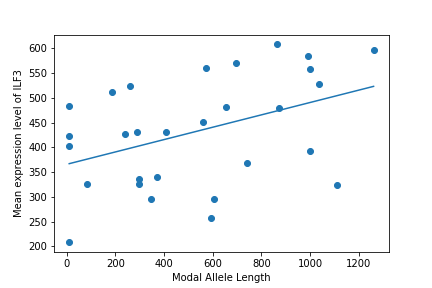
\includegraphics[width=135mm]{avgILF3.png}
	\caption{Mean expression level of Interleukin enhancer-binding factor 3 vs Modal Allele Length}
	\label{avgILF3}
\end{figure}

\subsubsection{Computing Differential Alternative Splicing Indicator} \label{subsection_DASI}

Likewise, for every probe in every probeset the difference between the mean expression level and the intensity measured at that probe can be computed, and plotted against Modal Allele Length. This is done in order to offset any possible differential expression which may be present in the gene of interest. The trend captured should be a direct indicator of DAS. Let us call such difference Differential Alternative Splicing Indicator (DASI).

The following 4 plots show such difference in expression in probeset 3820698, which correspond to exon 3820698.

\begin{figure}
	\centering
	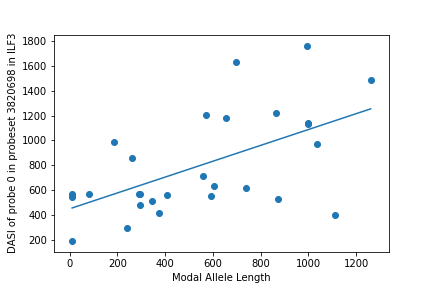
\includegraphics[width=135mm]{probeILF30.png}
	\caption{DASI of probe 1 in probeset 3820698 targeting an exon in ILF3 vs Modal Allele Length}
    \label{probeILF30}
\end{figure}

\begin{figure}
	\centering
	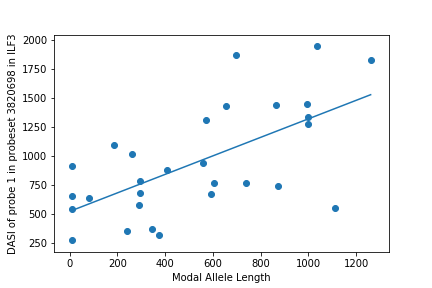
\includegraphics[width=135mm]{probeILF31.png}
	\caption{DASI of probe 2 in probeset 3820698 targeting an exon in ILF3 vs Modal Allele Length}
    \label{probeILF31}
\end{figure}

\begin{figure}
	\centering
	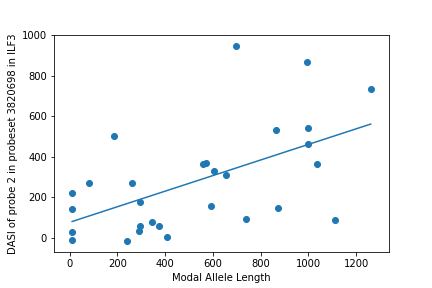
\includegraphics[width=135mm]{probeILF32.png}
	\caption{DASI of probe 3 in probeset 3820698 targeting an exon in ILF3 vs Modal Allele Length}
    \label{probeILF32}
\end{figure}

\begin{figure}
	\centering
	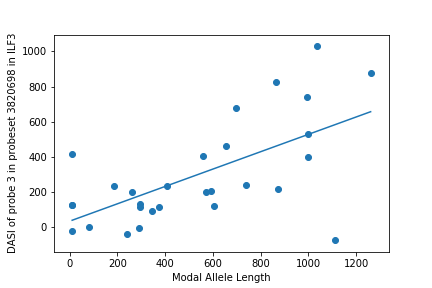
\includegraphics[width=135mm]{probeILF33.png} \caption{DASI of probe 4 in probeset 3820698 targeting an exon in ILF3 vs Modal Allele Length}
    \label{probeILF33}
\end{figure}

Putting aside issues around multiple hypothesis testing, exon targeted by probeset 3820698 can be regarded as differentially alternatively spliced, as patients with high MAL exhibit higher levels of expression at this exon relative to the total expression of the entire gene, a quantity measured by DASI. A likely explanation is that one or more isoforms containing the exon targeted by probeset 3820698 is preferentially expressed in DM1.

The effect of differential expression at this single exon can also be a possible cause of the slight differential expression of the entire gene (as seen in figure \ref{avgILF3}), as the high expression at this exon may significantly shift mean expression levels of the whole gene for patients with high MAL.

\subsubsection{Whole Genome Analysis of Alternative Splicing in DM1} \label{section_wholegenome}

In order to put the reasoning in subsection \ref{subsection_DASI} on a more rigorous footing we test against the null hypothesis that the best-fit line (as measured by minimising the sum of squares of residuals) of DASI vs modal allele length has slope 0. This line can be seen plotted for the exon targeted by probeset 3820698 in figures \ref{probeILF30}, \ref{probeILF31}, \ref{probeILF32}, \ref{probeILF33}. The p-values for null hypotheses that the slope of each respective regression line is 0 are respectively $7.72×10^{-4}$, $2.37×10^{-4}$, $1.84 × 10^{-3}$ and $2.64 × 10 ^{-4}$. (For reference, the p-value of a corresponding hypothesis for the slope of the best fit line of mean ILF3 expression vs MAL in figure \ref{avgILF3} is 0.0224.).

This computation results in up to $4$ p-values per each probeset, or equivalently, up to $4×n$ p-values per gene, where $n$ is the number of exons in that gene.

A subsequent challenge is combining these p-values into a single p-value per probeset, which can later undergo appropriate multiple testing correction procedure. We develop such method mathematically \ref{pvalues}. Unfortunately the method developed relies on the assumption of independence of individual p-values under the null hypothesis. This can not be guaranteed in our case, as each individual p-value is derived from a set of measurements of the same, unknown quantity, namely the cellular concentration of the transcription product of a give gene. Therefore Monte Carlo Simulation is applied to the statistic obtained from the mathematical approach in order to obtain the null distribution, and the p-value is retrieved directly from the result of the simulation.

Obtained p-values are corrected using the Benjamini-Hochberg procedure \parencite{Benjamini1995} and a list of genes with a given False Discovery Rate (FDR) is produced.

For any FDR < 0.11 the list of genes is empty. At FDR = 0.12, the list contains 5049 genes.

To test our findings against previously published research, we compare the list of 800 most significant genes from our list against the list of 40 genes whose splicing was previously identified as abnormal in DM1 by \cite{Nakamori2013}. Although the overlap between the two lists is a modest 7 genes, performing a hypergeometric test indicates that such overlap would be extremely unlikely to have occurred by chance, $p = 8.02 × 10^{-07}$. However, it is admittedly a poor scientific practice to arbitrarily fix a parameter of 800 most significant genes for the purpose of comparing the two lists (although the number was fixed \textit{a priori} rather than \textit{post hoc}). Work is being carried out to use a more appropriate rank-based test which will not need to assume such parameter.

\subsection{Method to combine multiple p-values coming from repetitions of the same experiment} \label{pvalues}

The approach described in this chapter was developed to cope with the challenge of combining multiple p-values coming from multiple repetitions of the same experiment, which arised in section \ref{section_wholegenome}.

\begin{definition}[Product Distribution with n degrees of freedom.]

Let $n$ be a positive integer, and $X$ be a random variable with
$$
X \sim
\begin{cases}
  \frac{(-log(x))^{n-1}}{(n-1)!} & \text{for } 0 < x \leq 1 \\
  0 & \text{otherwise } \\
\end{cases}
$$

Then, let us say that X follows a Product Distribution with $n$ degrees of freedom, or

$$X \sim \Prod(n)$$

\end{definition}

Let us verify that $\Prod(k)$ is well-defined. Direct computation with a Computer Algebra System shows that $$\int_{0}^{1}\Prod(k)=1$$ which suffices.

\begin{lemma}[Distribution of a product of uniformly distributed IIDs]

\label{lemmaProdUniform}

Let $X_{1}, X_{2}, ..., X_{n}$ be Identically and Independently Distributed (IID) random variables with $$X_{i} \sim \Uniform(0, 1)$$ Then we have that $$\prod_{i=1}^{i=n} X_{i} \sim \Prod(n)$$

\end{lemma}

\begin{proof}
By induction on $n$. For the base case let $n = 1$. From definition of $X_{1}$ we have that

$$ X_{1} \sim \Uniform(0, 1) $$

and from the definition of $\Uniform(0, 1)$ we have that

$$
X_{1} \sim \begin{cases}
  1 & \text{for } 0 \leq x \leq 1 \\
  0 & \text{for}
\end{cases}
$$

Since $X_{1}$ is continuously distributed we can change the value of the PDF at $x=0$ without changing the distribution. Hence

$$
X \sim
\begin{cases}
  \frac{(-log(x))^{0}}{(0)!} & \text{for } 0 \leq x \leq 1 \\
  0 & \text{otherwise } \\
\end{cases}
$$

And therefore $X_{1} \sim \Prod(1)$, as required. For the inductive step let us show that for any positive integer $k$, $X \sim \Prod(k)$, and $Y \sim \Uniform(0, 1)$ we have that $Z = Y * X \sim \Prod(k+1)$. Let us follow the method given by \cite{Wasserman2004} in the chapter "Transformation of Several Random Variables" to compute the Probability Distribution Function (PDF) of Z.

Let $x$, $y$, $z$ be the realizations of respectively $X$, $Y$, $Z$.

Let $F_{Z}$ be the Cumulative Distribution Function (CDF) of $Z$, and let $f_{Z}$ be the PDF of $Z$.

Let $f_{X,Y}$ be the joint probability distribution of $X$ and $Y$.

Let us first find the boundary of the region $A_{z} = \{(x, y): x * y \leq z\}$. Let us consider two cases $x \leq z$ and $x > z$. In the first case, the boundary will be given by extreme values of $x$ and $y$, $x \in [0, z]$, $y \in [0, 1]$. In the second case, the boundary will be given be the extreme value of $x$, $x \in [z, 1]$, by the extreme value of $y = 0$ from below, and by the function $y = z/x$ from above.

Let us denote the region enclosed by the boundary in the first case $L_{z}$, and in the second case $R_{z}$. We have that $L_{z} \cup R_{z} = A_{z}$.

Let us first compute $F_{Z}$. We have that
$$F_{Z} = \iint_{A_{Z}}f_{X,Y}\partial A_{Z}=\iint_{L_{Z}}f_{X, Y}\partial L_{Z} + \iint_{R_{Z}}f_{X, Y}\partial R_{Z}$$
Let us deal with each integral separately. In each case
$$f_{X, Y}=1f_{X}=\frac{(-log(x))^{k-1}}{(k-1)!}$$ since $X$ and $Y$ are independent, $Y \sim \Uniform(0, 1)$ and $A_{Z}$ is contained in the unit square with the bottom left corner at $(0, 0)$.

Direct computation using a CAS (TODO cite Wolfram Alpha) shows that $$\iint_{R_{Z}}f_{X, Y}\partial R_{Z}=\frac{z(-log(z))^{k}}{k!}$$

and $$\iint_{L_{Z}}f_{X, Y}\partial L_{Z}=\frac{\Gamma(k, -log(z))^{k}}{k!}$$ where $\Gamma$ is the upper incomplete gamma function. These can be differentiated over $z$ and summed to obtain $$f_{Z}=\frac{-log(z)^{k}}{k!} = \Prod(k+1)$$ both inside and outside $z \in [0, 1]$.

From the inductive assumption we have $\prod_{i=1}^{i=k} X_{i} \sim \Prod(k)$ and from the definition we have $X_{i+1} \sim \Uniform(0, 1)$. Using the derivation above we obtain $$\prod_{i=1}^{i=k+1} X_{i} \sim \Prod(k+1).$$
\end{proof}

\begin{definition}[AS Statistic]
Let $P = \{p_{1}, \ldots , p_{k}\}$ be p-values from independent statistical tests, all testing a given hypothesis. Let us define $\prod{p_{i}}$ to be the AS-statistic of $P$
\end{definition}

It is known that under the null hypothesis each each of $p_{i} \sim \Uniform(0, 1)$.

From lemma \ref{lemmaProdUniform} it follows that under the null hypothesis $\AS(\boldsymbol{P}) \sim \Prod{k}$. Given any realisation $a = \AS(\boldsymbol{P})$ we can compute

$$\alpha = \int_{0}^{a}\Prod(k)$$

and reject the null hypothesis at the confidence interval of $\alpha$, gaining control of type I error analogously to a p-value.

\section{Future Work}

We believe that the methods developed for effective detection of alternative splicing should be applicable to other datasets on Myotonic Dystrophy and to other similar diseases, such as Huntington Disease or perhaps even dissimilar diseases like hypertension. As such, we plan to apply them in the context of these diseases.

Likewise, we plan to test efficacy of Individual Specific Effects on these datasets to confirm our suspicion of the lack of efficacy.

\printbibliography
\end{document}
